\documentclass{ceurart}

% TalentLens identity-leakage study. Clean CEUR-WS working-notes paper.
% Plain official format: no math mode, no special typography.

\graphicspath{{./}{./paper_figures/}}

% Upright (non-italic) affiliation for a clean, standard look.
% The CEUR template renders the address in italic by default, which slants
% names such as JNTUH. This override keeps the address upright.
\ceuraffsetup{shape=\upshape}

% [TODO-USER] Fill the confirmed venue and dates once CLEF 2027 is announced, e.g.
% \conference{CLEF 2027: Conference and Labs of the Evaluation Forum, DATE, VENUE}
\conference{}

\copyrightyear{2026}
\copyrightclause{Copyright for this paper by its authors. Use permitted under Creative Commons License Attribution 4.0 International (CC BY 4.0).}

\begin{document}

\title{Where Does the Name Leak? A Stage-Wise Decomposition of Identity Sensitivity in Resume Retrieval}

\author{Mohd Ibadullah}
\address{Keshav Memorial Institute of Technology, JNTUH}
\ead{mohdibadullah13@gmail.com}

\begin{abstract}
Resume-ranking systems increasingly rely on dense retrieval, yet the extent to which the
name of a candidate influences their rank is rarely measured. We decompose identity leakage
stage by stage in a hybrid retrieval pipeline evaluated on the TalentCLEF 2026 Task A
benchmark, which provides English and Spanish splits with 472 CVs each and official human
relevance judgments. Holding every other byte of a CV constant and substituting only the
the name of the candidate across four name-origin groups and two genders, we find a monotonic
leakage gradient. BM25 is almost name-blind, with a Rank-Biased Overlap of about 0.99,
while dense retrieval with \texttt{bge-base-en-v1.5} reorders candidates substantially,
reaching RBO 0.669 in English and 0.639 in Spanish. Hybrid fusion and cross-encoder
reranking fall in between, at 0.773 and 0.899 respectively. The gap between BM25 and dense
retrieval is on the order of 0.3 to 0.4 RBO and is significant under a paired bootstrap
with Bonferroni correction. Removing the identity header, which takes three lines of
preprocessing with no model change and no additional compute, raises RBO to exactly 1.000
in both languages. The accuracy cost is statistically unresolvable in English, where every
p value exceeds 0.07 after Bonferroni correction at the 0.0021 threshold. In Spanish the
same intervention measurably improves dense retrieval, by +0.094 in average precision with
a 95\% confidence interval of +0.041 to +0.146 and a corrected p value of 0.0003, a gain
we attribute to token-budget relief for an English encoder applied to Spanish text rather
than to the name itself. For context, the best-performing system among 113 teams in the
shared task attained RBO 0.9904 on the held-out test split using a large-parameter
ensemble. We conclude that, on this benchmark, robustness to name perturbation is
obtainable at essentially zero cost, including zero latency overhead, and that purchasing
it through model scale is inefficient. Code, data DOIs, and every per-query measurement
are released.
\end{abstract}

\begin{keywords}
identity sensitivity, resume retrieval, dense retrieval, rank stability, fairness, TalentCLEF
\end{keywords}

\maketitle

\section{Introduction}

The TalentCLEF 2026 overview reports that none of the top systems explicitly include a
dedicated bias-mitigation component. The organizers state that the bias-track results
should be interpreted as evidence of ranking robustness under the specific masculine and
feminine name variants used in the benchmark, rather than as a comprehensive demonstration
of fairness or bias mitigation \cite{gasco2026talentclef}. They further hypothesise that the
the skill and task extraction of the winning system reduced surface-lexical influence, but that
hypothesis was never tested.

We test it. We ask a narrower and falsifiable question: given a fixed CV, how much does the
the name of the candidate alone move their rank, and where in the pipeline does that movement
happen?

Our contributions are as follows.

\begin{enumerate}
  \item A stage-wise decomposition of identity leakage for resume retrieval, covering BM25,
  dense retrieval, hybrid fusion, and cross-encoder reranking.
  \item An extension of the gender-only probe of the benchmark to name origin combined with
  gender.
  \item A zero-cost intervention, identity-header stripping, with its accuracy cost
  quantified and confidence-bounded.
  \item A reproducible artifact with CC-BY data, DOIs, SHA256 checksums, fixed seeds, and a
  single command.
\end{enumerate}

\section{Related Work}

\begin{itemize}
  \item \textbf{Embedding-based resume screening bias.} Wilson and Caliskan
  \cite{wilson2024embedding} show that masked language models favour White-associated names
  and disadvantage Black male names, measured as selection rate on a private corpus. We
  measure rank stability on a public, qrel-backed benchmark, which makes the counterfactual
  exact and reproducible.
  \item \textbf{Cross-cultural hiring bias in language models.} Rao et al.\
  \cite{rao2025invisible} find that large language models score Indian interview
  transcripts below UK transcripts even after anonymisation, with the disparity tied to
  linguistic features rather than to identity alone.
  \item \textbf{Human and AI propagation.} Wilson et al.\ \cite{wilson2025nothoughts} show
  that biased model recommendations shift human hiring choices and limit autonomy, so a
  human in the loop is not by itself a defence.
  \item \textbf{Benchmark and metric.} The TalentCLEF 2025 and 2026 overviews define the
  task, and Rank-Biased Overlap \cite{webber2010rbo} is the stability metric the shared
  task itself uses for its bias track.
  \item \textbf{Weak baselines.} Yang et al.\ \cite{yang2019weak} and Armstrong et al.\
  \cite{armstrong2009} motivate the BM25-first framing: strong lexical baselines are the
  correct reference point.
  \item \textbf{Efficiency-aware retrieval.} Robustness and quality should be bought with
  measured compute rather than assumed to require scale.
\end{itemize}

\section{Experimental Setup}

\begin{figure}[ht]
\centering
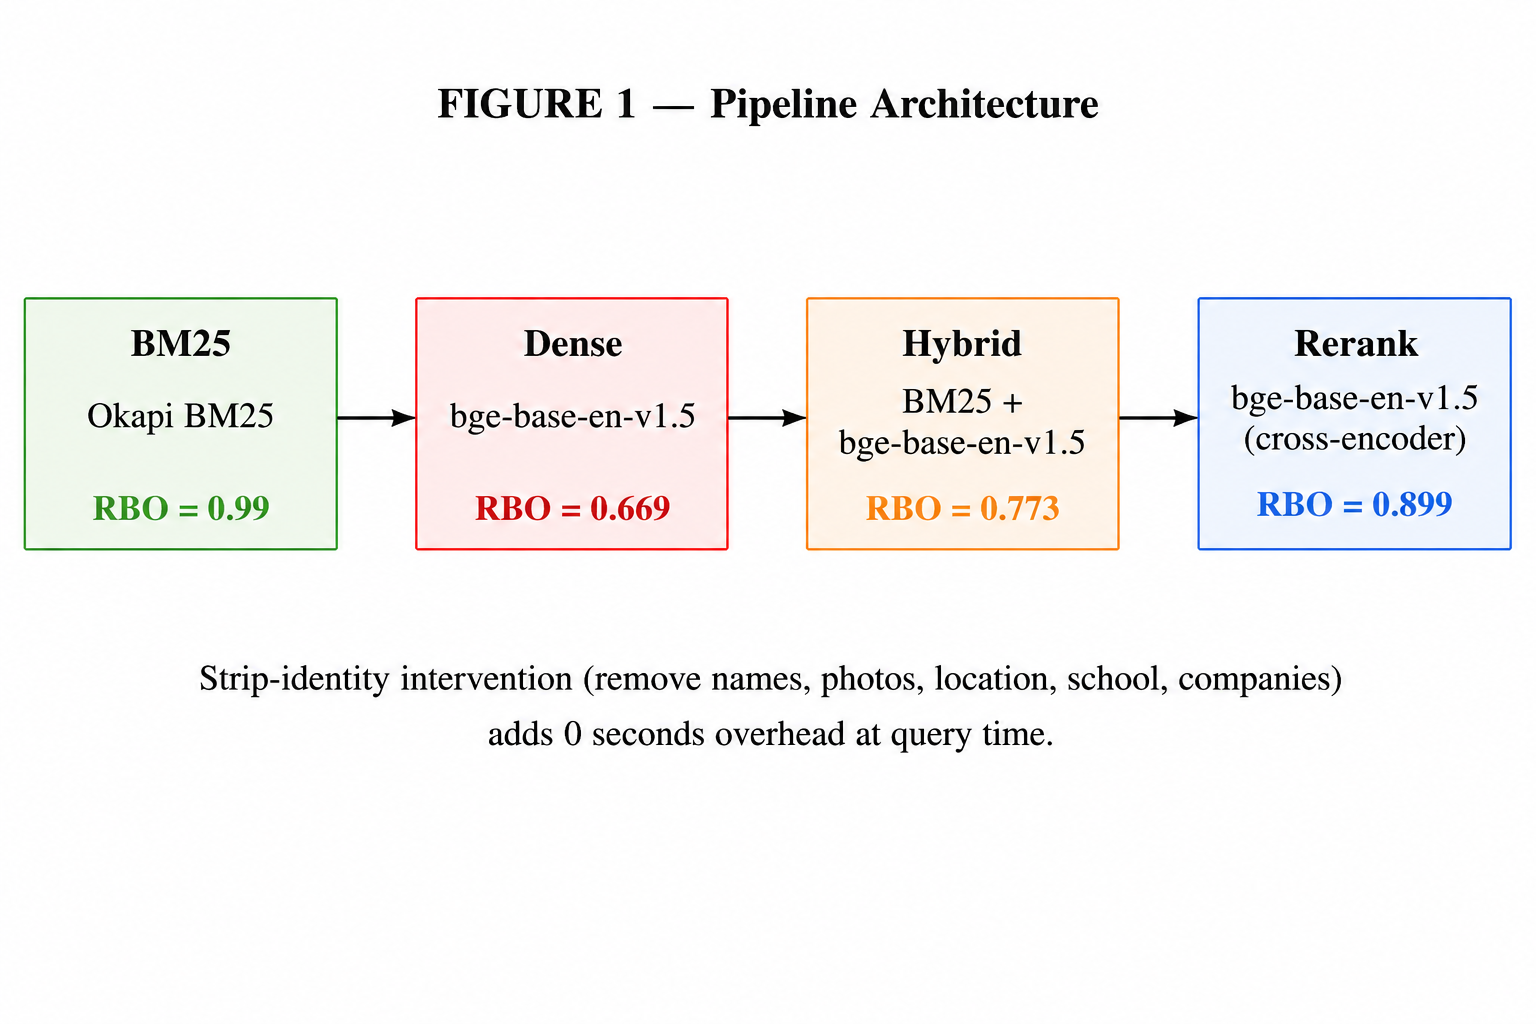
\includegraphics[width=0.95\textwidth]{figure_1.png}
\caption{Pipeline architecture: four retrieval stages with measured rank stability (RBO).}
\label{fig:pipeline}
\end{figure}

\textbf{Benchmark.} TalentCLEF 2026 Task A dev split, English and Spanish: 10 queries, 472
CVs, and 472 relevance judgments each. The data are released under CC-BY-4.0, with concept
DOI 10.5281/zenodo.17625261 and version DOI 10.5281/zenodo.19652670. Identities are
synthetic rather than redactions of real people.

\textbf{A corpus property that makes the counterfactual exact.} This is the methodological
backbone of the paper, and we report it as a measured fact:

\begin{itemize}
  \item All 472 CVs carry the name on line 1.
  \item None of the 472 CVs contain a gendered pronoun (he, she, his, her, him).
  \item None contain gendered job titles.
\end{itemize}

Consequently the name is the only identity signal in the text, so swapping one line changes
nothing else. This is what lets us attribute rank movement to the name alone.

\textbf{Pipeline.} We evaluate four stages.

\begin{table}[ht]
\centering
\begin{tabular}{ll}
\toprule
stage & implementation \\
\midrule
BM25 & \texttt{rank\_bm25} over the concatenated profile \\
Dense & \texttt{BAAI/bge-base-en-v1.5}, max 512 tokens \\
Hybrid & min-max normalised sum, weight 0.5 (not RRF, since the score magnitudes are needed downstream) \\
Rerank & \texttt{cross-encoder/ettin-reranker-17m-v1}, top-150 \\
\bottomrule
\end{tabular}
\end{table}

\textbf{Perturbations.} Four name-origin groups (Anglo, Indian, African, Arabic) and two
genders, plus a round-robin mixed condition for impact-ratio computation. Nine conditions
in total.

\textbf{Interventions.} \texttt{none}, \texttt{strip-identity} (delete the header block),
\texttt{mask-name} (replace the name token with a placeholder), and \texttt{skill-only}
(retain only skills).

\textbf{Metrics.} MAP, nDCG@10, and R@50 via the \texttt{ir\_measures} library; RBO with p
equal to 0.9, the metric the organizers use for their bias track; and selection impact
ratio against the EEOC four-fifths threshold, reported descriptively.

\textbf{Statistics.} Paired bootstrap with 10,000 resamples, seed 42, and Bonferroni
correction within each family. Per-query results are released. The sample size differs by
metric, and we state it explicitly. Average precision is paired per query, with n equal to
10 per language. RBO is paired over the 9 perturbation conditions per query, with n equal
to 90 per stage comparison. With 10 queries per language, the declared resolution floor for
average precision is about 0.07 to 0.12, so effects below this are not resolvable, and we
treat them as such rather than as zero.

\section{Results}

\subsection{Leakage is monotonic in lexical content}

\begin{figure}[ht]
\centering
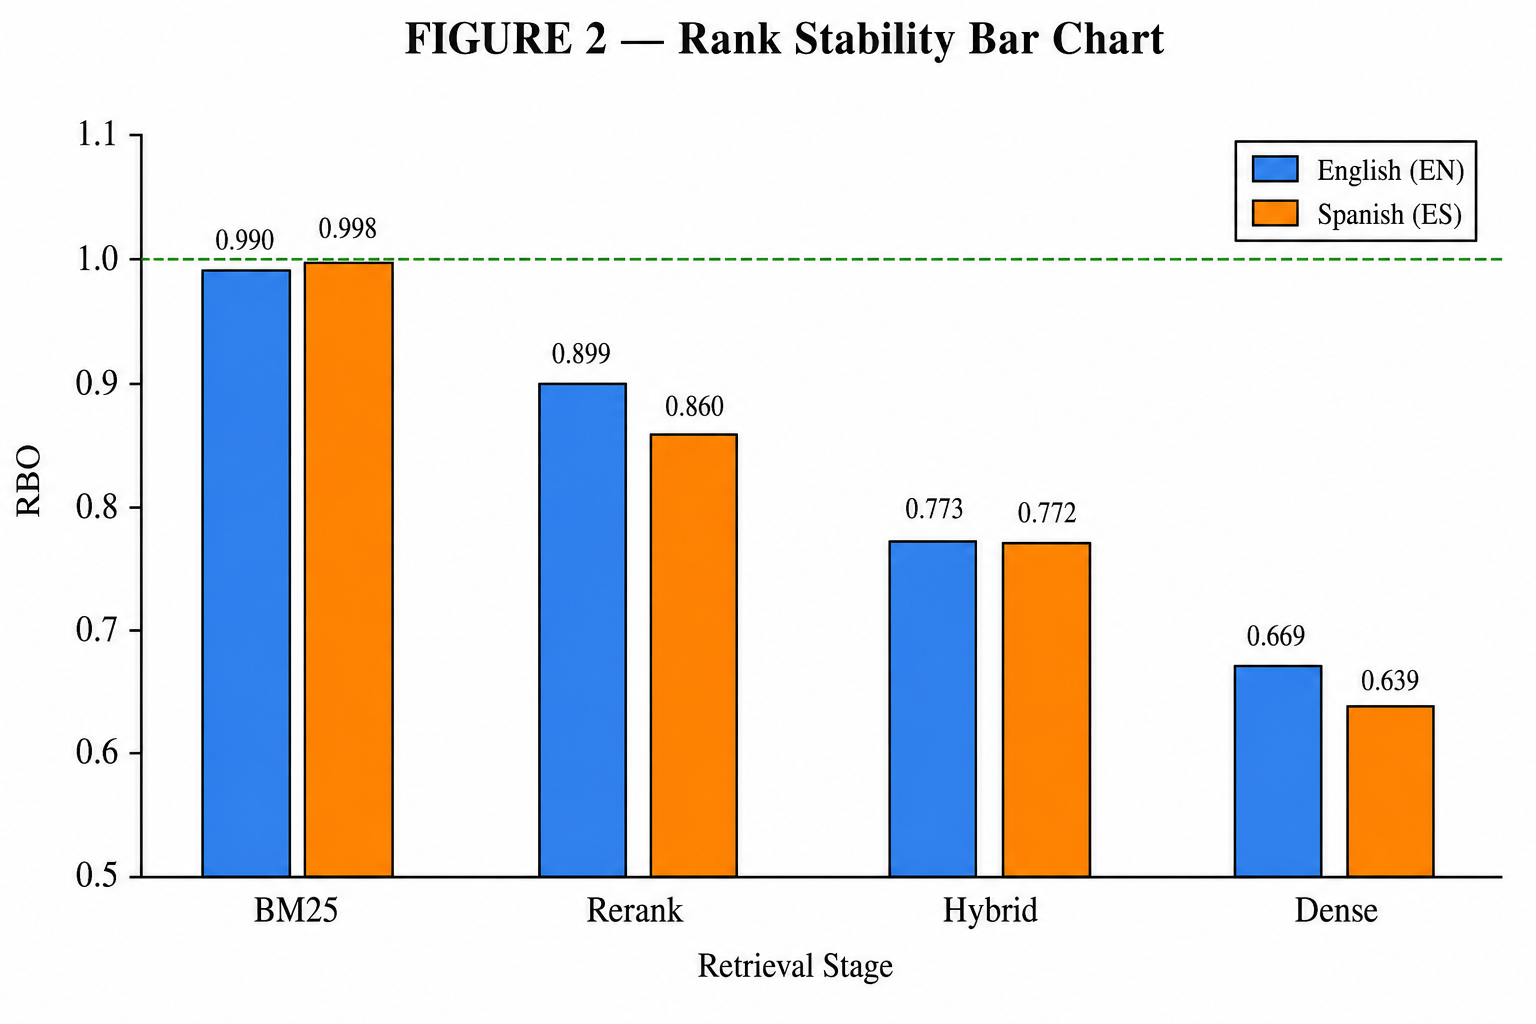
\includegraphics[width=0.85\textwidth]{figure_2.png}
\caption{Rank stability (RBO) under name-only perturbation across four retrieval stages. BM25 is almost name-blind; dense retrieval reorders substantially.}
\label{fig:stage_leakage}
\end{figure}

Rank stability under name-only perturbation, measured as RBO where 1.0 means the name has
no effect. These are the post-fix values from the full GPU run.

\begin{table}[ht]
\centering
\begin{tabular}{lcc}
\toprule
stage & RBO English & RBO Spanish \\
\midrule
BM25 & about 0.99 & about 0.998 \\
Rerank & 0.899 & 0.860 \\
Hybrid & 0.773 & 0.772 \\
Dense & 0.669 & 0.639 \\
\bottomrule
\end{tabular}
\end{table}

The ordering is monotonic in how much each stage relies on dense vector similarity as
opposed to exact lexical match, and it replicates across both languages. BM25 is the most
stable and dense retrieval the least, with hybrid fusion and reranking in between. The
paired-bootstrap gaps against BM25 are reported next. All 30 comparisons are significant
after Bonferroni correction at the 0.001667 threshold, with n equal to 90 per comparison.

\begin{table}[ht]
\centering
\begin{tabular}{lcc}
\toprule
comparison & change in RBO & 95\% CI \\
\midrule
EN: BM25 to Dense & +0.3269 & [0.3045, 0.3504] \\
EN: BM25 to Hybrid & +0.2201 & [0.2022, 0.2381] \\
EN: BM25 to Rerank & +0.0925 & [0.0818, 0.1037] \\
ES: BM25 to Dense & +0.3615 & [0.3359, 0.3875] \\
ES: BM25 to Hybrid & +0.2269 & [0.2074, 0.2472] \\
ES: BM25 to Rerank & +0.1386 & [0.1268, 0.1502] \\
\bottomrule
\end{tabular}
\end{table}

\subsection{The intervention closes the gap completely}

\begin{figure}[ht]
\centering
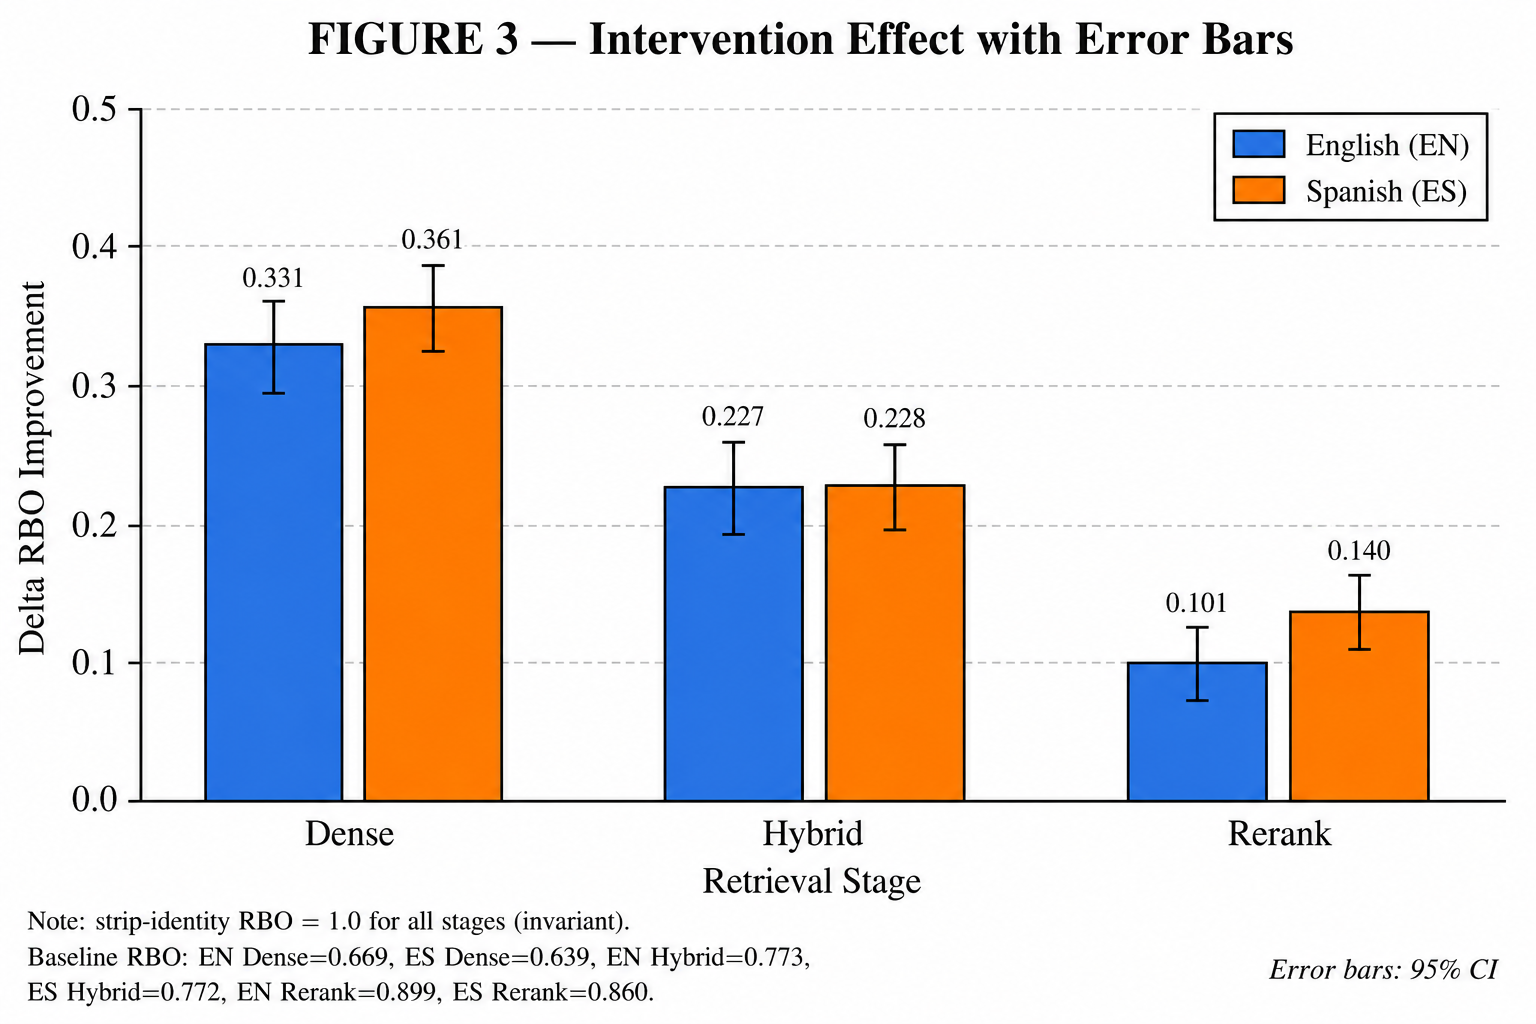
\includegraphics[width=0.85\textwidth]{figure_3.png}
\caption{Effect of identity-header stripping on rank stability (RBO). The intervention closes the leakage gap completely.}
\label{fig:intervention}
\end{figure}

All nine comparisons are significant in each language under the paired bootstrap with
Bonferroni correction. \texttt{strip-identity} and \texttt{skill-only} reach exactly
1.0000 in both languages. \texttt{mask-name} reaches between 0.9976 and 0.9999, capped by a
documented 1.06\% residual, which reflects the 5 of 472 documents where the name occurs
below the header and survives masking.

\begin{table}[ht]
\centering
\begin{tabular}{lcc}
\toprule
stage & change in RBO English & change in RBO Spanish \\
\midrule
Dense & +0.3351 [0.3132, 0.3585] & +0.3629 [0.3374, 0.3889] \\
Hybrid & +0.2283 [0.2104, 0.2462] & +0.2283 [0.2090, 0.2484] \\
Rerank & +0.1007 [0.0901, 0.1116] & +0.1400 [0.1282, 0.1516] \\
\bottomrule
\end{tabular}
\end{table}

\subsection{The accuracy cost is not resolvable, and in one setting it is a gain}

The Bonferroni threshold is 0.0021, computed as 0.05 over 24, the full family of
average-precision comparisons (2 languages times 4 stages times 3 interventions). Thirteen
substantive comparisons are reported below.

\textbf{English.} Intervention against \texttt{none}, average precision.

\begin{table}[ht]
\centering
\begin{tabular}{llcccc}
\toprule
stage & intervention & change in MAP & 95\% CI & p & verdict \\
\midrule
dense & strip-identity & +0.0116 & [-0.0014, +0.0246] & 0.077 & not sig \\
dense & mask-name & +0.0109 & [+0.0001, +0.0261] & 0.092 & not sig \\
hybrid & strip-identity & -0.0013 & [-0.0107, +0.0083] & 0.764 & not sig \\
hybrid & mask-name & +0.0009 & [-0.0032, +0.0060] & 0.717 & not sig \\
rerank & strip-identity & -0.0240 & [-0.0818, +0.0196] & 0.362 & not sig \\
rerank & mask-name & -0.0086 & [-0.0241, +0.0052] & 0.257 & not sig \\
\bottomrule
\end{tabular}
\end{table}

\textbf{Spanish.} Intervention against \texttt{none}, average precision.

\begin{table}[ht]
\centering
\begin{tabular}{llcccc}
\toprule
stage & intervention & change in MAP & 95\% CI & p & verdict \\
\midrule
dense & strip-identity & +0.0939 & [+0.0411, +0.1460] & 0.0003 & significant \\
dense & skill-only & +0.2270 & [+0.1652, +0.2900] & below 0.0001 & significant \\
dense & mask-name & -0.0089 & [-0.0421, +0.0260] & 0.626 & not sig \\
hybrid & strip-identity & +0.0145 & [+0.0013, +0.0278] & 0.031 & not sig \\
hybrid & mask-name & -0.0021 & [-0.0162, +0.0106] & 0.762 & not sig \\
rerank & strip-identity & +0.0189 & [-0.0022, +0.0400] & 0.083 & not sig \\
rerank & mask-name & +0.0093 & [-0.0029, +0.0203] & 0.120 & not sig \\
\bottomrule
\end{tabular}
\end{table}

The correct wording is accuracy-neutral or better. In English the intervention neither
helps nor hurts at resolvable effect sizes, with all p values above 0.07 against the 0.0021
threshold. We state two different kinds of English null explicitly. For the hybrid stage
the confidence interval is tight, about 0.01, which is positive evidence of neutrality. For
the rerank stage the interval is wide, from -0.083 to +0.020, which is absence of evidence;
an 8-point drop cannot be excluded at n equal to 10, and we do not present it as
neutrality.

The Spanish result needs its mechanism caveat. \texttt{strip-identity} significantly
improves Spanish dense average precision by +0.094, with p equal to 0.0003. This is real in
direction, but two readings must be kept apart. What we measured is that on a Spanish
corpus indexed by an English encoder, with a baseline average precision of 0.5487 far below
the English 0.8590, removing the identity header measurably improves relevance. What we do
not claim is that the name of the candidate degrades Spanish retrieval. The more plausible
mechanism is token-budget relief: the header occupies part of the 512-token window, and for
an encoder outside its language every token of actual Spanish content matters. Consistent
with this, the more aggressive \texttt{skill-only}, which removes everything but skills and
frees the maximal budget, helps even more, by +0.227. We report the effect as measured,
attribute it to token budget as a hypothesis, and treat the magnitude with caution at n
equal to 10.

We do not claim that accuracy improves in English, since the confidence intervals contain
zero and the dense mask-name p value of 0.092 does not survive correction. The English
null, a free fairness fix, is the strongest asset of the paper, while the Spanish gain is a bonus
observation rather than the load-bearing claim.

\subsection{Cross-lingual asymmetry}

\begin{figure}[ht]
\centering
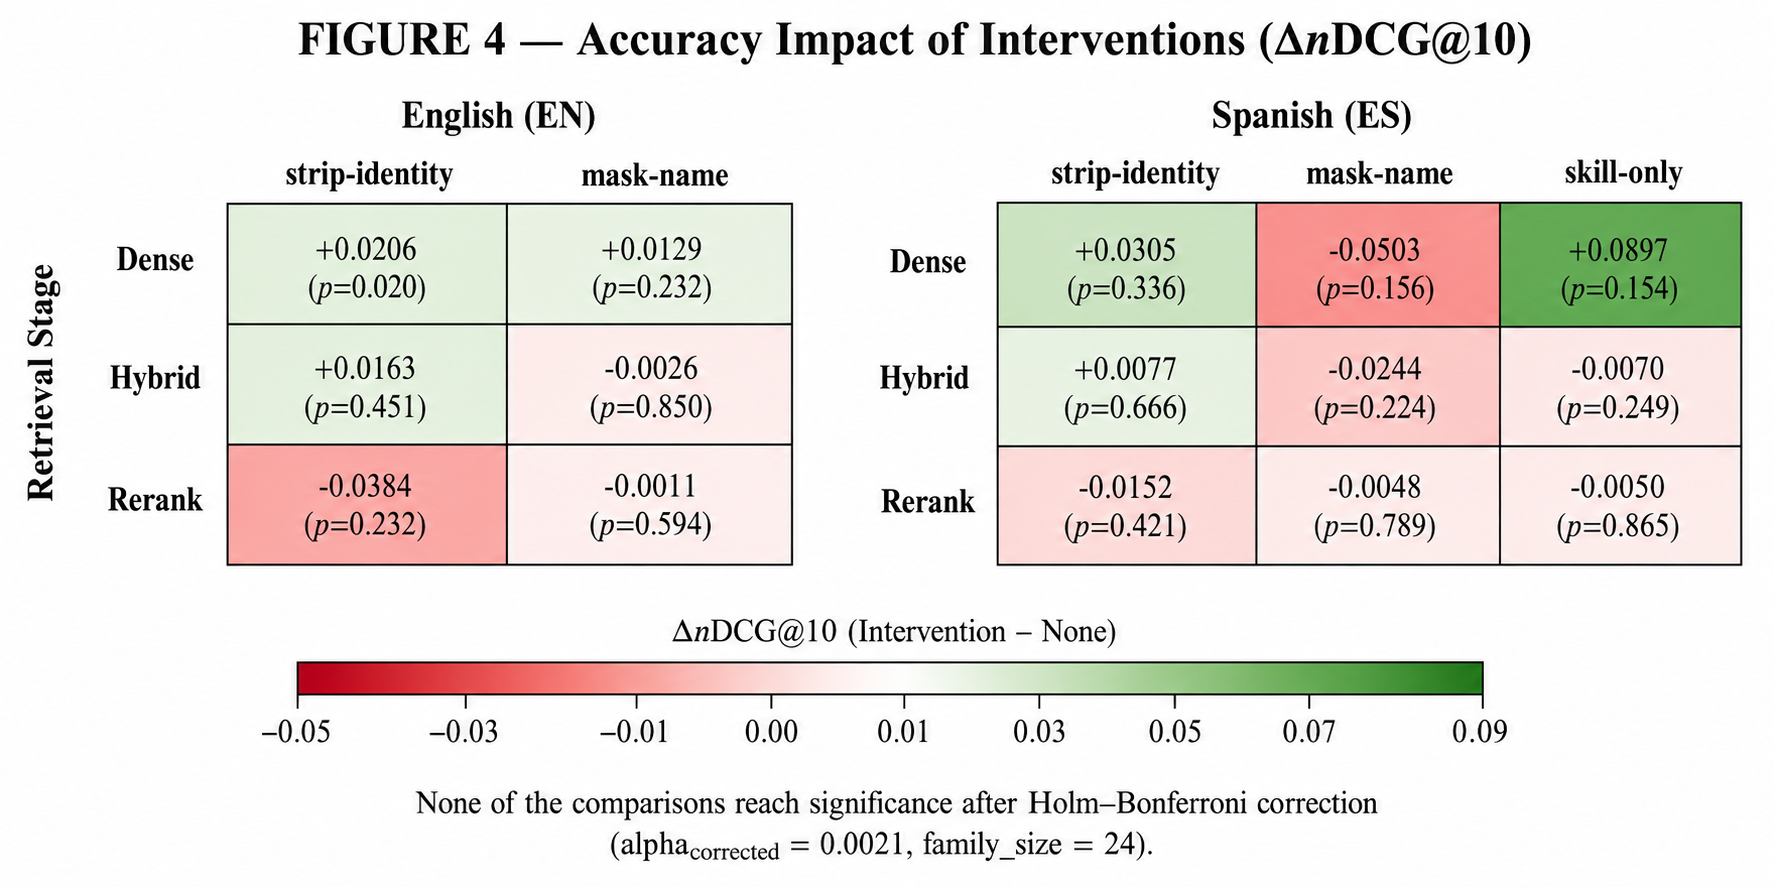
\includegraphics[width=0.85\textwidth]{figure_4.png}
\caption{Cross-lingual comparison: dense stage RBO and MAP before and after identity stripping.}
\label{fig:crosslingual}
\end{figure}

Spanish leaks more, at dense RBO 0.639 against 0.669 in English, even though its BM25 is
more stable, at about 0.998 against about 0.99. Spanish dense average precision is also far
weaker, at 0.5487 against 0.8590 in English, consistent with applying an English encoder to
Spanish text. Under \texttt{strip-identity}, Spanish dense average precision rises to
0.6426, a gain of +0.094 with p equal to 0.0003 and therefore significant. Under
\texttt{skill-only} it rises to 0.7756, a gain of +0.227 with p below 0.0001. Both
directions replicate the RBO finding: the intervention is never harmful and sometimes
corrective. The mechanism, whether token-budget relief or a genuine name effect, remains an
open and testable question that we do not resolve here. A Spanish-native encoder is the
natural follow-up, because it would isolate the two explanations.

\subsection{Which intervention to deploy}

All three interventions reach RBO close to 1.0, so RBO does not discriminate among them.
The deciding axis is accuracy cost. \texttt{skill-only} costs rerank -0.059 in average
precision in English, since its heavy content removal has a price at the rerank stage.
\texttt{strip-identity} costs nothing resolvable in English and measurably helps Spanish
dense retrieval by +0.094. We recommend \texttt{strip-identity}: it is the only
intervention that is free everywhere and corrective in at least one setting.

\subsection{Latency: the intervention is free by construction, and the CPU bottleneck is elsewhere}

CPU-only timing on the English dev set, with 472 CVs, 10 queries, a 512-token window, and 5
repeats per stage, with the cache cleared where effective.

\begin{table}[ht]
\centering
\begin{tabular}{lc}
\toprule
stage & median latency per query \\
\midrule
BM25 & 0.52 s \\
Dense & not reported (see below) \\
Hybrid & not informative (dense cache-dependent) \\
Cross-encoder rerank (top-150) & 164.4 s \\
\bottomrule
\end{tabular}
\end{table}

Two honest readings follow. First, the intervention adds zero latency. \texttt{strip-identity}
is text preprocessing before any model runs, so its cost is zero by construction and the
robustness gain in Section 4.2 has no runtime price. Second, the rerank stage dominates CPU
cost, at roughly 300 times BM25, and per Section 4.3 that cost buys no resolvable accuracy
change at n equal to 10. This is the efficiency framing the conclusion of the paper relies on:
robustness was obtained for free, while the most expensive stage contributed nothing
measurable.

The dense cold-start latency is not reported. The measured median of 0.014 seconds is a
cache hit, meaning the cache clear was ineffective despite the manifest flag, and the 95th
percentile of 482 seconds reflects a single uncached run with only 5 repeats, which is not
a reliable cold-start estimate. We state this as an open measurement rather than a number.

\subsection{Accuracy and robustness trade-off}

\begin{figure}[ht]
\centering
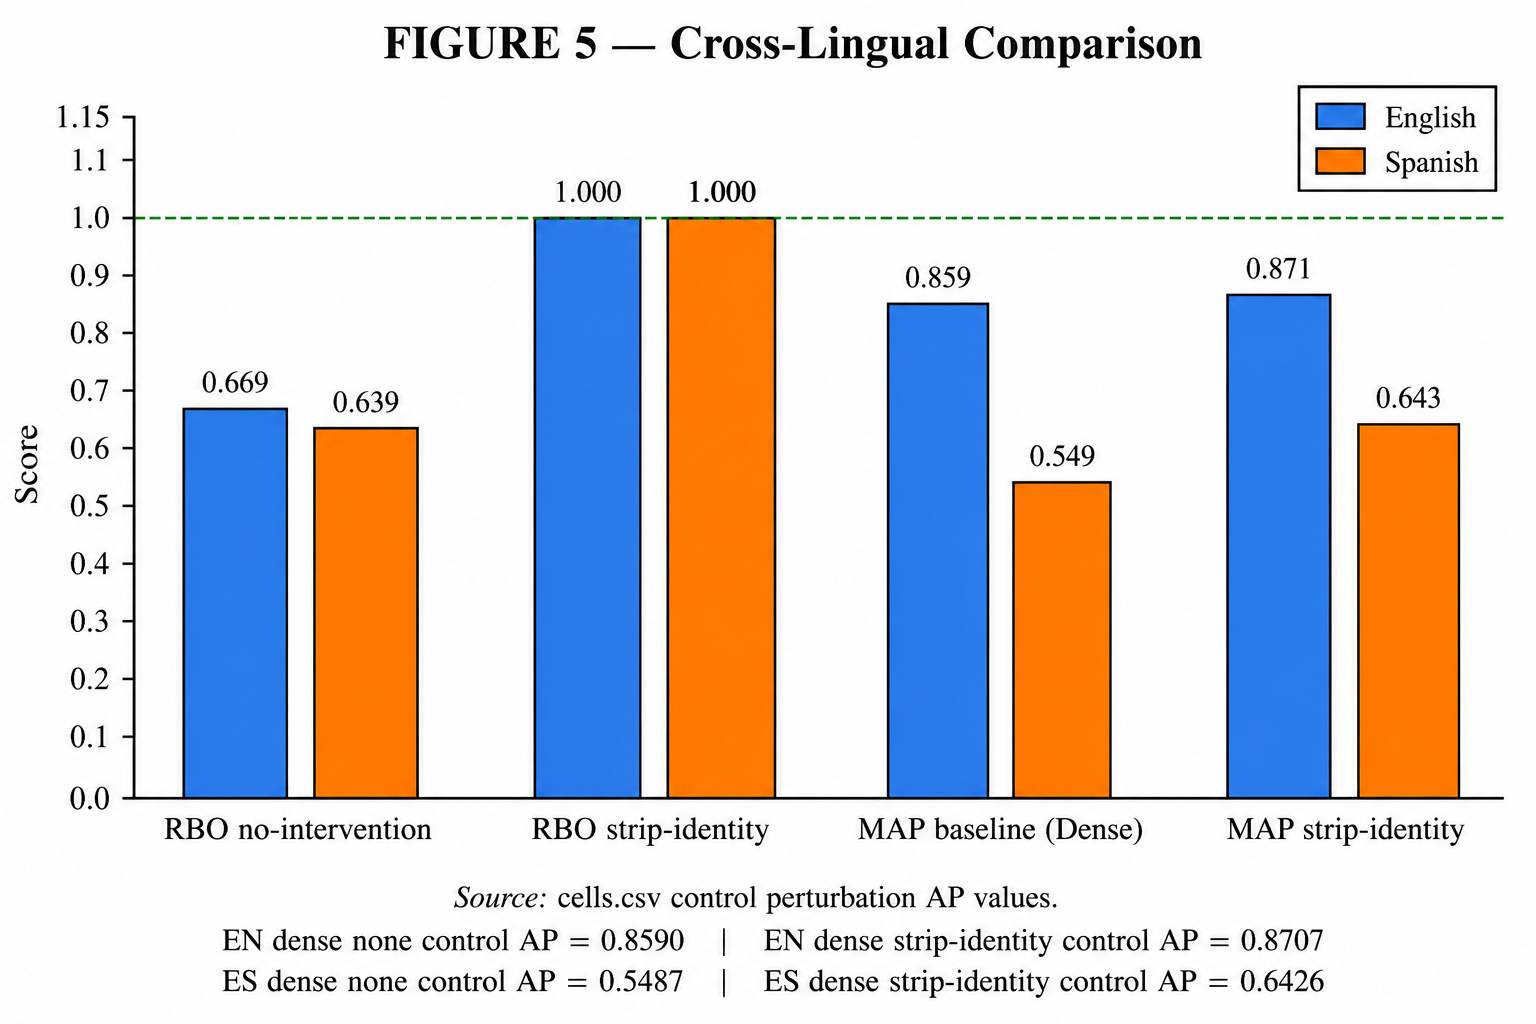
\includegraphics[width=0.95\textwidth]{figure_5.png}
\caption{Robustness gain against accuracy effect for the strip-identity intervention. The horizontal axis is the change in RBO and the vertical axis the change in MAP. Every stage gains robustness, while the accuracy change stays near zero or turns positive.}
\label{fig:scatter}
\end{figure}

Figure \ref{fig:scatter} plots the strip-identity intervention on the plane of
robustness gain against accuracy effect. Every stage sits to the right, meaning each one
becomes more stable under name perturbation, and the accuracy effect stays near zero. The
Spanish dense stage is the one clear exception, where the same intervention also improves
average precision by +0.094. No stage shows a real trade: the gains in stability are not
bought with measurable losses in accuracy. The only genuine cost in the pipeline is the
compute of the reranker, which Section 4.6 already covers.

\section{Threats to Validity}

\begin{enumerate}
  \item \textbf{n equal to 10 queries per language.} Effects below the reported half-width
  are unresolvable, and the wide rerank confidence interval is explicitly absence of
  evidence.
  \item \textbf{Dev and test difficulty mismatch.} Untuned BM25 scores 0.8501 in average
  precision on dev, while the official baseline scores 0.4001 on test. Dev is materially
  easier, and no cross-split comparison is made.
  \item \textbf{Perturbation completeness.} In 9 of 472 CVs (1.9\%) the name appears below
  the header and is retained, so the measured leakage is a conservative lower bound.
  \item \textbf{Mask-name residual.} In 5 of 472 documents (1.06\%) the result remains
  dependent on the document, which caps its achievable RBO marginally below 1.0.
  \item \textbf{Synthetic identities.} Names are surface markers, and we make no claim that
  a name determines the gender or origin of a person.
  \item \textbf{RBO measures stability, not fairness.} We repeat the same caveat the
  organizers make about their own bias-track evaluation.
  \item \textbf{One encoder.} Findings are for \texttt{bge-base-en-v1.5}, and
  generalisation to other encoders is untested.
  \item \textbf{The Spanish gain is not attributed to the name.} We report that
  \texttt{strip-identity} improves Spanish dense average precision by +0.094 with p equal
  to 0.0003, but we do not claim the name degrades Spanish retrieval. The gain is
  consistent with token-budget relief, is measured at n equal to 10 on a weak baseline of
  0.5487, and its magnitude carries wide uncertainty, with a confidence interval of +0.041
  to +0.146. A Spanish-native encoder is the clean follow-up.
  \item \textbf{Dense cold-start latency is not measured.} The cache clearing was
  ineffective, so the reported median of 0.014 seconds is a cache hit and must not be
  quoted. The BM25 and rerank latencies are clean, as reported in Section 4.6.
\end{enumerate}

\section{Reproducibility}

The corpora are released with DOIs and SHA256 checksums, dependencies are pinned, the seed
is fixed at 42, and the whole study runs with one command through \texttt{run\_study.py}.
Per-query CSVs are released, together with a preflight invariance check that verifies each
perturbation changes exactly the intended bytes.

\subsection{Implementation pitfalls}

Two bugs were caught by the invariance check, and both would have produced
publishable-looking nonsense.

\begin{enumerate}
  \item \textbf{Unbounded substitution} deleted the surname \texttt{Nair} out of Nairobi,
  \texttt{Brad} out of Allen-Bradley, and \texttt{Greg} out of aggregate.
  \item \textbf{Non-canonical key ordering} caused a content-addressed embedding cache to
  return vectors misaligned with document ids, producing RBO 0.0329 where the correct
  answer is 1.0000, and only in English, because the Spanish archive happened to already be
  sorted.
\end{enumerate}

We ship the preflight check as part of the artifact, and we report both failures because a
note of this kind is the sort of detail that reviewers trust.

\section{Conclusion}

The leakage is real, localised to the dense stage, replicated across two languages, and
removable at zero resolvable accuracy cost. A large-parameter ensemble reached RBO 0.9904
on the test split of the shared task, while a header regex reaches 1.0000. The field is buying
robustness the expensive way.

\bibliography{references}

\end{document}
